%%%%%%%%%%%%%%%%%%%%%%%%%%%%%%%%%%%%%%%%%%%%%%%%%%%%%%%%%%%%%%%%%%%%%%
\section{Microbenchmarks}\label{sec:eva-micro}
%%%%%%%%%%%%%%%%%%%%%%%%%%%%%%%%%%%%%%%%%%%%%%%%%%%%%%%%%%%%%%%%%%%%%%

In this section, we analyze the performance of the adaptation approaches
by utilizing several microbenchmarks from the aspects of overhead,
threshold quantification and the adaptation improvement respectively.

\subsection{Overhead Analysis}
We first evaluate the overhead of the user-guided approach and the
self-profiling based approaches for each window collective synchronization
call on a single node with one ghost process and increasing number of local
processes. For user-guided approaches that only insert hint at window
allocation, the names are abbreviated to CSP(U, <ON, OFF>) in which ON or
OFF is the hint passed through window info; similarly, CSP(U-coll, <ON, OFF>)
is denoted for the user-guided modes that also insert hint in fence or the
MPI\_WIN\_SET\_INFO; for self-profiling based approaches, CSP(P) is denoted
for the mode that only allows user-handled synchronization, and CSP(GP)
is for the mode that also allows ghost-offloaded synchronization for
PUT/GET operations.

Figure~\ref{fig:eva-micro-overhead-alloc} shows the overhead of
\fn{MPI\_WIN\_ALLOCATE}. When the asynchronous progress is enabled,
Casper always experience substantial cost in the window allocation time,
since we have to create internal windows and exchange internal information
globally. This can be shown as the gap between CSP(U, ON) and the original
MPI; the performance of CSP(U, OFF) is very close to that of the original
MPI, because we do not perform additional processing and return immediately
when the asynchronous progress in the window is disabled; the
CSP(U-coll, ON) and CSP(P) approaches perform the same processing as that
for CSP(U, ON) thus deliver the same performance. We note that the CSP(GP)
mode always updates the local ghost cache, however, it is not significant
since the overhead of GET\_ACCUMUALTE on shared memory is too small.
We omit CSP(U-coll, OFF) in this graph, because it performs the same processing that in CSP(U-coll, ON).


Figure~\ref{fig:eva-micro-overhead-fence} compares the overhead of each
approach at fence call. For CSP(U, ON), it does not perform adaptation
in fence, the additional cost comparing to original MPI is because of
the passive-mode translation in our Casper implementation as already
discussed in our previous work; the CSP(U-coll, ON) approach only updates
local window since the user hint is consistent on all processes, thus
showing similar cost as that of CSP(U, ON); the CSP(P) approach, however,
need to perform the user synchronization that exchanges the status of
local asynchronous progress among processes; the CSP(GP) approach needs to also update the data in every local ghost cache after user synchronization,
thus consistently showing close to 1$\mu$s overhead comparing to CSP(P).


Figure~\ref{fig:eva-micro-overhead-setinfo} compares the overhead of each
approach at window info setting with symmetric hint. Similar as the fence
call, both CSP(U, ON) and CSP(U-coll, ON) do not involve any additional
communication; the self-profiling based approaches have to always perform
additional all-to-all communication, thus showing increasing overhead
with increase of processes. The additional 1$\mu$s overhead of
CSP(GP) comparing to CSP(P) is the same as we have explained in fence.


\begin{figure*}[ht]
\centering
\subfigure[Window allocation]{
  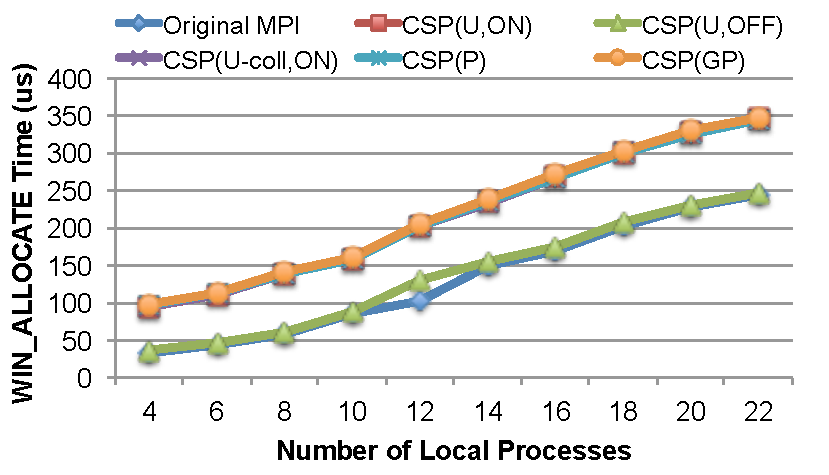
\includegraphics[width=0.64\columnwidth]{figures/adpt-casper/eva_edison_overhead_adpt_alloc_n1.pdf}
  \label{fig:eva-micro-overhead-alloc}
}
\subfigure[Fence]{
  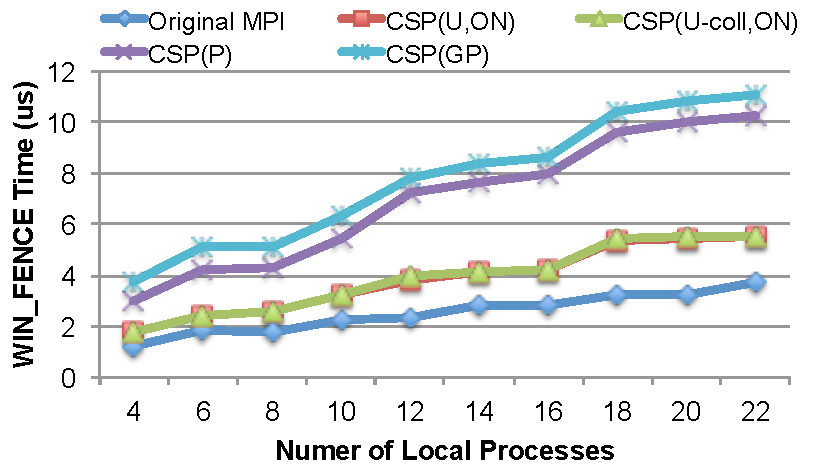
\includegraphics[width=0.64\columnwidth]{figures/adpt-casper/eva_edison_overhead_adpt_fence_n1.pdf}
  \label{fig:eva-micro-overhead-fence}
}
\subfigure[Window info setting with symmetric]{
  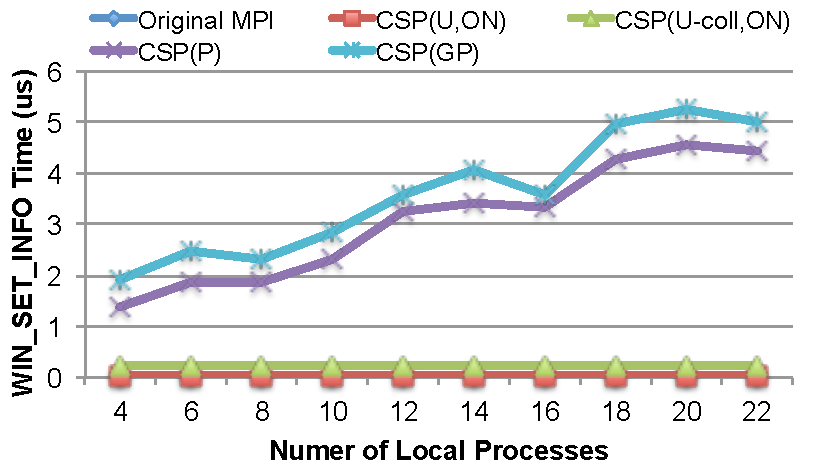
\includegraphics[width=0.64\columnwidth]{figures/adpt-casper/eva_edison_overhead_adpt_setinfo_n1.pdf}
  \label{fig:eva-micro-overhead-setinfo}
}
\caption{Adaptation Overhead at Window Collective Synchronization.}
\label{fig:eva-micro-overhead-coll}
\end{figure*}


\subsection{Self-Profiling based Prediction}

As we have discussed in Section~\ref{sec:des-adpt-p-pred},
the prediction step follows the notion that the asynchronous progress may
not be needed if the communication frequency is high on the target process.
However, such frequency can be artificially high if most cost of the MPI
calls is caused by the internal instructions rather than that spends
in message waiting. In this section, we compare the communication frequency
and the needs of asynchronous progress determined in following scenarios.


\subsubsection{Increasing Number of Operations}
Figure~\ref{fig:eva-micro-thresh-freq-nop} shows the measurements
with increasing number of operations in all-to-all RMA communication
on 2 nodes with 22 user processes and 2 ghost processes per node.
Every user process performs \emp{lockall,alltoall-N[get,flush],computation,unlockall}
pattern, in which \emp{N} indicates the number of operations and the
computation is demonstrated as 5000$\mu$ busy waiting. We compare the
performance and the communication frequency measured within asynchronous
progress (ON) and without asynchronous progress (OFF).
Withing increasing number of operations, every process also becomes
more frequently making progress since it waits on every single GET
operation. The speedup of asynchronous progress gradually reduces and
becomes negative from 32 operations because of both reduced needs of
asynchronous progress and the load imbalance issue among large number
of operations. Furthermore, we notice that the frequency of the
asynchronous progress disabled case (FREQ(OFF)) is much higher than
that in the enabled case (FREQ(ON)) when the number of operations is
small, this is because the communication overhead is significantly
higher in the disabled case due to lack of asynchronous progress.

\subsubsection{Increasing Number of Processes}
Figure~\ref{fig:eva-micro-thresh-freq-ppn} shows a similar experiment,
but scales the number of local processes while keeping the number of
GET operations at 100. Similar as the trend in the previous experiment,
the speedup of asynchronous progress reduces with increasing number of
local processes, and eventually becomes negative at 12 local processes.
The reason is similar as the first experiment, the number of operations
and flush calls issued on every process is increasing following the
increase of processes, thus allowing every process to frequently stay
inside MPI in order to make progress. Meanwhile, the overhead caused by
load imbalance in the asynchronous progress enabled case is increasing
with larger number of local processes, since every ghost process has to
serve more user processes.

\subsubsection{Increasing Size of Operations}
Our third experiment uses yet another variant of the first experiment
by varying the size of the operation while keeping the number of
operations at 10. Every process performs ACCUMULATE operations
following the same pattern with 5000$\mu$ busy waiting.
Figure~\ref{fig:eva-micro-thresh-freq-ppn} shows the results.
This case, however, shows different trend of speedup comparing to the
previous experiments, although the frequency of communication is still
increasing following with the scaling of operation size. This is because
the overhead of heavy accumulation operation (i.e., in the receiving
process on target side for internode operation, and the sending process
to local target process) are increasing with the size of operation and
consistently dominates the communication time taken on every process.
\mynote{add proportion of accumulation overhead in graph.}

\begin{figure*}[ht]
\centering
\subfigure[Increasing number of operations]{
  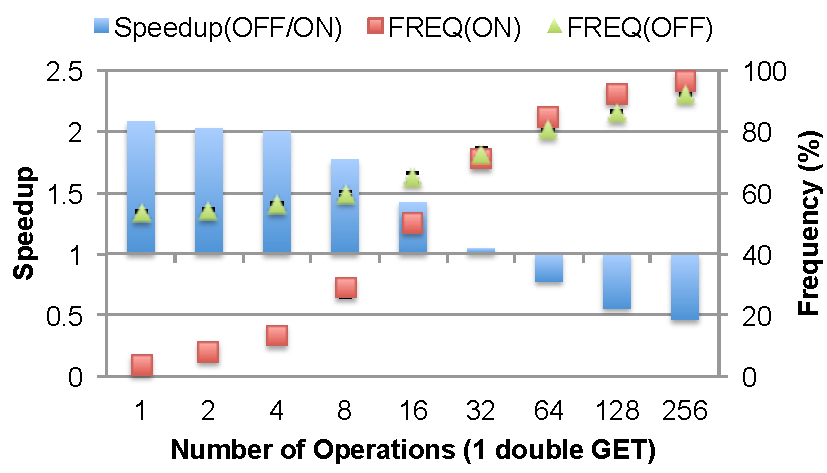
\includegraphics[width=0.64\columnwidth]{figures/adpt-casper/eva_edison_thresh_freq_nop_n2.pdf}
  \label{fig:eva-micro-thresh-freq-nop}
}
\subfigure[Increasing number of processes]{
  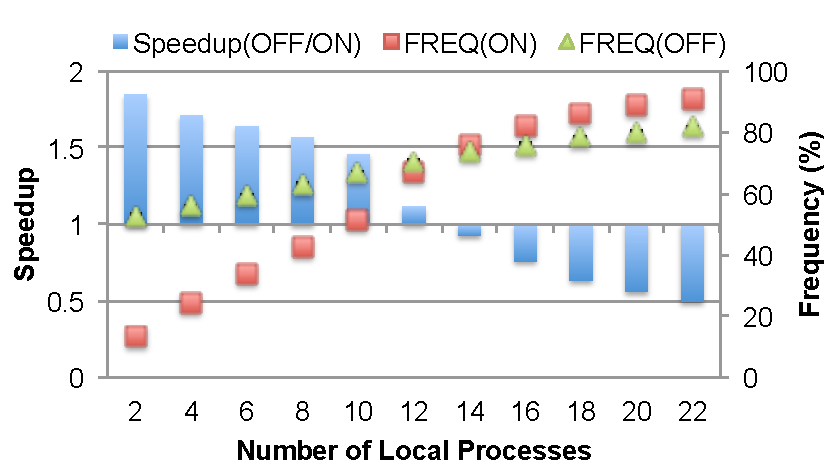
\includegraphics[width=0.64\columnwidth]{figures/adpt-casper/eva_edison_thresh_freq_ppn_n2.pdf}
  \label{fig:eva-micro-thresh-freq-ppn}
}
\subfigure[Increasing operation size]{
  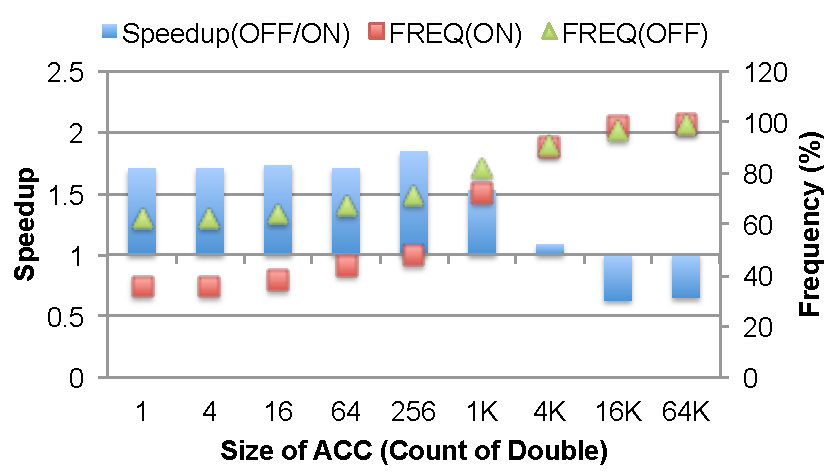
\includegraphics[width=0.64\columnwidth]{figures/adpt-casper/eva_edison_thresh_freq_opsize_n2.pdf}
  \label{fig:eva-micro-thresh-freq-opsz}
}
\caption{Efficiency of Asynchronous Progress related to Communication Frequency.}
\label{fig:eva-micro-thresh-freq}
\end{figure*}


\subsection{Adaptation Improvement}
\mynote{Prediction only focuses on the needs of asynchronous progress,
addressing the load imbalance issue is an additional benefit, but should
not be the data being predicted.}

\mynote{show what \libname(static, dynamic) can improve, cannot improve.}